\section{Theoretical Analysis}
\label{sec:analysis}

In this section, the circuit shown in Figure~\ref{fig:circuit} is analysed
theoretically. We will begin by analyzing the circuit by applying the Mesh Method and, after that, we will analyze it again using the Nodal Method . In order to this, we will use Kirchhoff's circuit laws (KVL and KCL) together with Ohm's Law to obtain the theoretical results.

Note that we defined one of the nodes as GND, which is the central node of the circuit, 
having then randomly assigned numbers to the remaining ones. This will help us to
later simulate the circuit and perform its analysis.

 
\subsection{Mesh Method}

--- A mesh is a loop that contains no other loops. ---
The Mesh Method consists of assigning a current with a certain direction to each loop in a circuit, as shown in Figure~\ref{fig:mcurrents}, and then evaluating the circuit based on the new currents defined.

\begin{figure}[h!] \centering
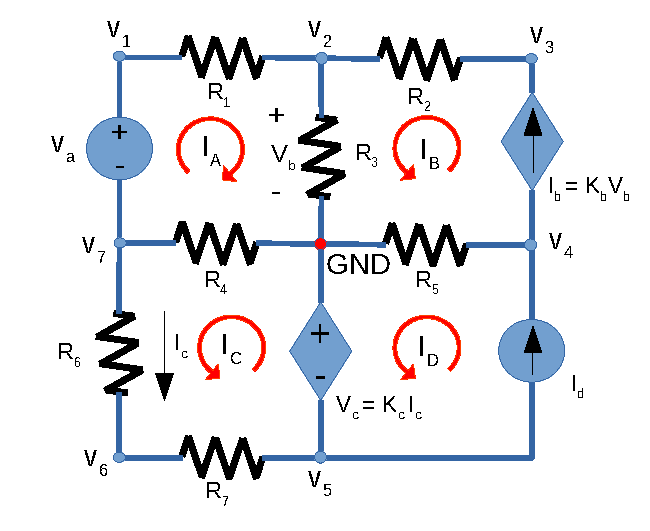
\includegraphics[width=0.4\linewidth]{mcurrents.pdf}
\caption{Circuit with each mesh current clockwise or counterclockwise direction assigned, to assist in the analysis of the circuit by the Mesh Method.}
\label{fig:mcurrents}
\end{figure}

In this way, the KVL equations are applied to loops which do not have current sources or whose current is not known.

\textit{Equations obtained to:}

\textit{Mesh A}
\begin{equation}
  -V_a+ R_1\cdot I_A + R_3 \cdot (I_A+I_B)+ R_4 \cdot (I_A+I_C) =0
  \label{eq:kvl}
\end{equation}

\textit{Mesh B}
\begin{equation}
  I_B = I_b = K_b \cdot V_b = K_b \cdot R_3 \cdot (I_A + I_B)
  \label{eq:kvl2}
\end{equation}

\textit{Mesh C}
\begin{equation}
  I_C=I_c
  \label{eq:kvlaux}
\end{equation}
\begin{equation}
  R_4 \cdot (I_C + I_A) + R_6 \cdot I_C + R_7 \cdot I_C - K_c \cdot I_C = 0
  \label{eq:kvl3}
\end{equation}

\textit{Mesh D}
\begin{equation}
  I_D =I_d
  \label{eq:kvl4}
\end{equation}

Then, the equations are solved in order to obtain the currents of each mesh. \vspace {1cm}

\textit{Matricial Equation obtained:}
\begin{gather}
	\begin{bmatrix}
		R_1 + R_3 + R_4 & R_3 & R_4 & 0  \\
		K_b \cdot R_3 & K_b \cdot R_3 - 1& 0 & 0 \\
		R_4 & 0 & R_4 + R_6 + R_ 7 - K_c & 0 \\
		0 & 0 & 0 & 1 \\
	\end{bmatrix}
	\begin {bmatrix} I_A \\ I_B \\ I_C \\ I_D \end{bmatrix}
	=
	\begin {bmatrix} V_a \\ 0 \\ 0 \\ I_d \end{bmatrix}
\end{gather}

The solution of this matricial equation is determined by Octave:

\begin{table}[H]
  \centering
  \begin{tabular}{|l|r|}
    \hline    
    {\bf Mesh Current} & {\bf Ampere[A]} \\ \hline
    $I_{A}$ & 2.015673e-03 \\ \hline
$I_{B}$ & -2.109620e-03 \\ \hline
$I_{C}$ & -1.157872e-03 \\ \hline
$I_{D}$ & 1.040860e-03 \\ \hline

  \end{tabular}
  \caption{Mesh Current Values}
  \label{tab:mesh}
\end{table}

Knowing these currents, it is possible to determine any nodal voltages and branch currents, using Ohm’s Law.

\begin{equation}
  I_C=I_c
\end{equation}
\begin{equation}
  V_c=K_c\cdot I_c
\end{equation}
\begin{equation}
  V_b=R_3\cdot (I_A+I_B)
\end{equation}
\begin{equation}
  I_b=K_b\cdot V_b
\end{equation}
\begin{equation}
  I_{R1}=I_A
\end{equation}
\begin{equation}
  I_{R2}=I_B
\end{equation}
\begin{equation}
  I_{R3}=I_A+I_B 
\end{equation}
\begin{equation}
  I_{R4}=I_A+I_C
\end{equation}
\begin{equation}
  I_{R5}=I_B - I_D
\end{equation}
\begin{equation}
  I_{R6}=I_C
\end{equation}
\begin{equation}
  I_{R7}=I_C
\end{equation}

\begin{table}[H]
  \centering
  \begin{tabular}{|l|r|}
    \hline    
    {\bf Name} & {\bf Ampere[A] or Volt[V]} \\ \hline
    $V_{b}$ & -2.924287e-01 \\ \hline
$I_{b}$ & -2.109620e-03 \\ \hline
$V_{c}$ & -9.279827e-06 \\ \hline
$I_{c}$ & -1.157872e-03 \\ \hline
$I_{R1}$ & 2.015673e-03 \\ \hline
$I_{R2}$ & -2.109620e-03 \\ \hline
$I_{R3}$ & -9.394704e-05 \\ \hline
$I_{R4}$ & 8.578007e-04 \\ \hline
$I_{R5}$ & -3.150480e-03 \\ \hline
$I_{R6}$ & -1.157872e-03 \\ \hline
$I_{R7}$ & -1.157872e-03 \\ \hline

  \end{tabular}
  \caption{Voltages and currents of some circuit components}
  \label{tab:valm}
\end{table}
 
\subsection{Nodal Method}

--- Nodes connect components in a circuit ---
The Nodal Method consists of choosing a reference node against which all other voltages are measured. Through the KCL equations and other additional equations, it is possible to determine the voltage at each node.

\begin{figure}[H] \centering
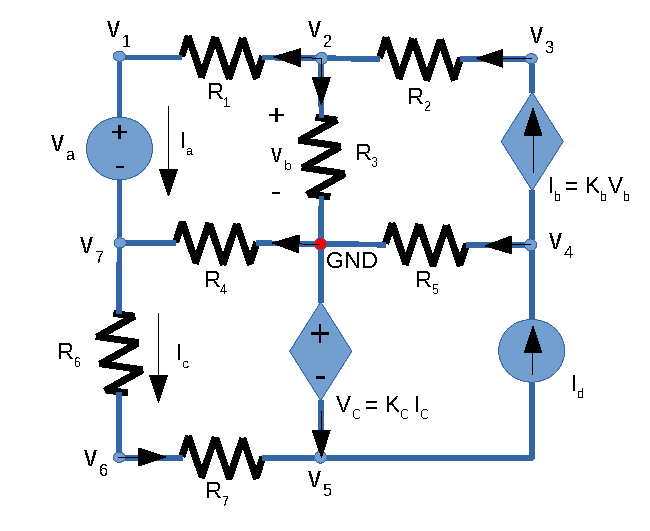
\includegraphics[width=0.4\linewidth]{nvoltages.pdf}
\caption{Circuit with each current direction arbitrarily assigned, to assist in the analysis of the circuit by the Nodal Method.}
\label{fig:nvoltages}
\end{figure}

It was assigned potencial 0 to the central node in order to proceed with the analysis. Because of that, we can write:

\begin{equation}
  V_b=V_2 - 0 = V_2
\end{equation}
\begin{equation}
  I_b= K_b \cdot V_b= K_b \cdot V_2
\end{equation}

We first start by calculating the values of the conductances of the various resistors:

\begin{equation}
  G_i=1/R_i
\end{equation}

Then we determine the equations obtained by applying KCL in nodes not connected to voltage sources:

\textit{Node number 2}
\begin{equation}
  -(V_2 -V_1)\cdot G_1 -V_b \cdot G_3 + (V_3-V_2)\cdot G_2 =0 
  \Leftrightarrow V_1\cdot G_1+V_2 \cdot (-G_1-G_2-G_3) + V_3\cdot G_2 =0
  \label{eq:kcl2}
\end{equation}

\textit{Node number 3}
\begin{equation}
  I_b - (V_3-V_2) \cdot G_2=0 \Leftrightarrow V_2(G_2 + K_b) - G_2 \cdot V_3 =0
  \label{eq:kcl3}
\end{equation}

\textit{Node number 4}
\begin{equation}
  -(V_4-0) \cdot G_5+I_d-K_b\cdot V_2=0 \Leftrightarrow -K_b\cdot V_2-V_4 \cdot G_5 = -I_d
  \label{eq:kcl4}
\end{equation}

\textit{Node number 6}
\begin{equation}
 	V_5 \cdot G_7 + V_6\cdot (-G_6 -G_7) + V_7 \cdot G_6 =0
  \label{eq:kcl6}
\end{equation}

However, we need additional equations for nodes related to voltage sources:

\textit{Node number 1}
\begin{equation}
  (V_2 - V_1)\cdot G_1 -I_a =0 \Leftrightarrow I_a=(V_2 - V_1)\cdot G_1
  \label{eq:kcl}
\end{equation}

\textit{Node number 7}
\begin{equation}
  V_1 \cdot G_1 - G_1 \cdot V_2 - G_6 \cdot V_6 + V_7 \cdot (G_4 + G_6)=0
  \label{eq:kcl7}
\end{equation}

\textit{Equation (\ref{eq:kcl})+(\ref{eq:kcl7})}
\begin{equation}
  V_1\cdot G_1+V_2\cdot (-G_1)+V6\cdot (-G_6)+V_7\cdot (G_4+G_6)=0
  \label{eq:kcl17}
\end{equation}

\textit{Another additional Equations:}
\begin{equation}
  V_a=V_1-V_7
  \label{eq:kcl8}
\end{equation}
\begin{equation}
  0-V_5=K_c\cdot G_6\cdot (V_7-V_6) \Leftrightarrow V_5+V_6\cdot K_c\cdot (-G_6)+V_7\cdot K_c\cdot G_6=0
  \label{eq:kcl9}
\end{equation}

Matricial equation obtained using the nodal method:

\begin{gather}
	\begin{bmatrix}
		G_1 & -G_1 & 0 & 0 & 0 & -G_6 & G_4 + G_6 \\
		G_1 & -G_1 - G_2 - G_3 & G_2 & 0 & 0 & 0 & 0 \\
		0 & G_2 + K_b & -G_2 & 0 & 0 & 0 & 0 \\
		0 & K_b & 0 & G_5 & 0 & 0 & 0 \\
		0 & 0 & 0 & 0 & G_7 & -G_6 - G_7 & G_6 \\
		1 & 0 & 0 & 0 & 0 & 0 & -1 \\
		0 & 0 & 0 & 0 & 1 & -G_6\cdot K_c & G_6\cdot K_c \\
	\end{bmatrix}
	\begin {bmatrix} V_1 \\ V_2 \\ V_3 \\ V_4  \\ V_5 \\ V_6 \\ V_7 \end{bmatrix}
	=
	\begin {bmatrix} 0  \\ 0  \\ 0  \\ I_d \\ 0  \\ V_a \\ 0 \end{bmatrix}
\end{gather}

The solution of this matricial equation is determined by Octave:

\begin{table}[H]
  \centering
  \begin{tabular}{|l|r|}
    \hline    
    {\bf Node} & {\bf Voltage[V]} \\ \hline
    $V_{1}$ & 1.726209e+00 \\ \hline
$V_{2}$ & -2.924287e-01 \\ \hline
$V_{3}$ & -4.528138e+00 \\ \hline
$V_{4}$ & 9.535580e+00 \\ \hline
$V_{5}$ & 9.279827e-06 \\ \hline
$V_{6}$ & -1.191502e+00 \\ \hline
$V_{7}$ & -3.522212e+00 \\ \hline

  \end{tabular}
  \caption{Nodal Voltages Values}
  \label{tab:nodal}
\end{table}

Knowing these voltages, it is also possible to determine any components' voltages, by subtracting the voltages of each node where the component is connected, and branch currents, using Ohm’s Law.

\begin{equation}
  I_c=(V_7-V_6)\cdot G_6
\end{equation}
\begin{equation}
  V_c=K_c\cdot I_c
\end{equation}
\begin{equation}
  V_b=V_2
\end{equation}
\begin{equation}
  I_b=K_b\cdot V_b
 \end{equation}
 
 \begin{table}[H]
  \centering
  \begin{tabular}{|l|r|}
    \hline    
    {\bf Name} & {\bf Value [A or V]} \\ \hline
    $V_{b}$ & -2.924287e-01 \\ \hline
$I_{b}$ & -2.109620e-03 \\ \hline
$V_{c}$ & -9.279827e-06 \\ \hline
$I_{c}$ & -1.157872e-03 \\ \hline
$I_{R1}$ & -2.015673e-03 \\ \hline
$I_{R2}$ & -2.109620e-03 \\ \hline
$I_{R3}$ & -9.394704e-05 \\ \hline
$I_{R4}$ & 8.578007e-04 \\ \hline
$I_{R5}$ & 3.150480e-03 \\ \hline
$I_{R6}$ & -1.157872e-03 \\ \hline
$I_{R7}$ & -1.157872e-03 \\ \hline

  \end{tabular}
  \caption{Voltages and currents of some circuit components}
  \label{tab:valn}
\end{table}
